\documentclass[oneside,13pt,a4paper]{report}

% Chargement d'extensions
\usepackage[utf8]{inputenc}
\usepackage[french]{babel}
% csquotes va utiliser la langue définie dans babel
\usepackage[babel=true]{csquotes}
\usepackage[T1]{fontenc}
\usepackage{graphicx}
\usepackage[top=3cm, bottom=3cm, left=3cm, right=3cm]{geometry}
\usepackage{amsmath}
\usepackage{amssymb}


% Liens et autres
\usepackage{hyperref}
\hypersetup{
    colorlinks=true,
    linkcolor=black,
	urlcolor=blue,
	pdftitle={Rendu},
	bookmarks=true,
}

% Bout de code
\usepackage{listings}
\usepackage{color}

\definecolor{mygreen}{rgb}{0,0.6,0}
\definecolor{mygray}{rgb}{0.5,0.5,0.5}
\definecolor{mymauve}{rgb}{0.58,0,0.82}

\lstset{
  backgroundcolor=\color{white},   % choose the background color; you must add \usepackage{color} or \usepackage{xcolor}; should come as last argument
  basicstyle=\footnotesize,        % the size of the fonts that are used for the code
  breakatwhitespace=false,         % sets if automatic breaks should only happen at whitespace
  breaklines=true,                 % sets automatic line breaking
  captionpos=b,                    % sets the caption-position to bottom
  commentstyle=\color{mygreen},    % comment style
  deletekeywords={...},            % if you want to delete keywords from the given language
  escapeinside={\%*}{*)},          % if you want to add LaTeX within your code
  extendedchars=true,              % lets you use non-ASCII characters; for 8-bits encodings only, does not work with UTF-8
  firstnumber=0,                   % start line enumeration with line 1000
  frame=single,	                   % adds a frame around the code
  keepspaces=true,                 % keeps spaces in text, useful for keeping indentation of code (possibly needs columns=flexible)
  keywordstyle=\color{blue},       % keyword style
  %language=C++,                    % the language of the code
  morekeywords={*,...},            % if you want to add more keywords to the set
  numbers=left,                    % where to put the line-numbers; possible values are (none, left, right)
  numbersep=5pt,                   % how far the line-numbers are from the code
  numberstyle=\tiny\color{mygray}, % the style that is used for the line-numbers
  rulecolor=\color{black},         % if not set, the frame-color may be changed on line-breaks within not-black text (e.g. comments (green here))
  showspaces=false,                % show spaces everywhere adding particular underscores; it overrides 'showstringspaces'
  showstringspaces=false,          % underline spaces within strings only
  showtabs=false,                  % show tabs within strings adding particular underscores
  stepnumber=1,                    % the step between two line-numbers. If it's 1, each line will be numbered
  stringstyle=\color{mymauve},     % string literal style
  tabsize=2,	                   % sets default tabsize to 2 spaces
  literate=
  {á}{{\'a}}1 {é}{{\'e}}1 {í}{{\'i}}1 {ó}{{\'o}}1 {ú}{{\'u}}1
  {Á}{{\'A}}1 {É}{{\'E}}1 {Í}{{\'I}}1 {Ó}{{\'O}}1 {Ú}{{\'U}}1
  {à}{{\`a}}1 {è}{{\`e}}1 {ì}{{\`i}}1 {ò}{{\`o}}1 {ù}{{\`u}}1
  {À}{{\`A}}1 {È}{{\'E}}1 {Ì}{{\`I}}1 {Ò}{{\`O}}1 {Ù}{{\`U}}1
  {ä}{{\"a}}1 {ë}{{\"e}}1 {ï}{{\"i}}1 {ö}{{\"o}}1 {ü}{{\"u}}1
  {Ä}{{\"A}}1 {Ë}{{\"E}}1 {Ï}{{\"I}}1 {Ö}{{\"O}}1 {Ü}{{\"U}}1
  {â}{{\^a}}1 {ê}{{\^e}}1 {î}{{\^i}}1 {ô}{{\^o}}1 {û}{{\^u}}1
  {Â}{{\^A}}1 {Ê}{{\^E}}1 {Î}{{\^I}}1 {Ô}{{\^O}}1 {Û}{{\^U}}1
  {Ã}{{\~A}}1 {ã}{{\~a}}1 {Õ}{{\~O}}1 {õ}{{\~o}}1
  {œ}{{\oe}}1 {Œ}{{\OE}}1 {æ}{{\ae}}1 {Æ}{{\AE}}1 {ß}{{\ss}}1
  {ű}{{\H{u}}}1 {Ű}{{\H{U}}}1 {ő}{{\H{o}}}1 {Ő}{{\H{O}}}1
  {ç}{{\c c}}1 {Ç}{{\c C}}1 {ø}{{\o}}1 {å}{{\r a}}1 {Å}{{\r A}}1
  {€}{{\euro}}1 {£}{{\pounds}}1 {«}{{\guillemotleft}}1
  {»}{{\guillemotright}}1 {ñ}{{\~n}}1 {Ñ}{{\~N}}1 {¿}{{?`}}1
}

% Commande pour notation 'NB :' (nota bene)
\newcommand\nb[1][0.3]{N\kern-#1emB : }

% Espacement entre les paragraphes
\parskip=5pt

% pour afficher Schéma au lieu de figure dans les legende des images
\addto\captionsfrench{\def\figurename{Schéma}}

% Informations le titre, le(s) auteur(s), la date
\title{TITRE}
\author{
    Belkassim BOUZIDI \and
    Mélissa DADI  \and
    Chakib ELHOUITI \and
    Massili KEZZOUL \and
    Ramzi ZEROUAL
}
\date{\today}


\begin{document}
%\maketitle
\begin{titlepage}
	\centering
	{\scshape\LARGE Universite de Montpellier\par}
	{\scshape\Large Rapport de projet\par}
	\vspace{1.5cm}
	{\huge\bfseries TITRE\par}
	\vspace{2cm}
	{\Large\itshape
		Belkassim BOUZIDI \\
    Mélissa DADI \\
		Chakib ELHOUITI \\
		Massili KEZZOUL \\
		Ramzi ZEROUAL \\
		\par}

	\vspace{1.5cm}

	{\Large\itshape
		Encadrant :\par
		M\up{r} Pascal \textsc{Poncelet}
		\par}

	\vspace{2cm}

	\begin{figure}[h]
		\begin{minipage}[c]{.46\linewidth}
			\centering
			
\includegraphics[width=1\textwidth]{img/univ-montpellier.png}
		\end{minipage}
		\hfill%
		\begin{minipage}[c]{.46\linewidth}
			\centering
			
\includegraphics[width=1\textwidth]{img/fds.png}
		\end{minipage}
	\end{figure}

	\par\vspace{1cm}

	\vfill

	% Bottom of the page
	{\large \today\par}
\end{titlepage}

% ------------------------------------- %
% Introduction
% ------------------------------------- %

\parskip=5pt
\chapter*{Remerciements}
\vspace{\stretch{1}}
\begin{center}

	Tout d'abord nous souhaitons adresser nos remerciements au corps professoral et administratif de la faculté des sciences de Montpellier qui déploient des efforts pour assurer à leurs étudiants une formation actualisée.

	En second lieu, nous tenons à remercier notre encadrant M\up{r} Pascal \textsc{Poncelet} pour ses précieux conseils et son aide durant toute la période de travail.

	Nos vifs remerciements vont également aux membres du jury pour l’intérêt qu’ils ont porté à notre projet en acceptant d’examiner notre travail.

	Nous remercions M\up{r} Yahia Zeroual pour sa relecture attentive de ce rapport.

\end{center}
\vspace{\stretch{1}}

\parskip=0pt
\tableofcontents

% Espacement entre les paragraphes
\parskip=5pt

% ------------------------------------- %
% Organisation
% ------------------------------------- %

\chapter{Organisation du projet}
\section{Méthodes d’organisation}

Afin de mener à bien le développement du projet, nous avons décidé de travailler un maximum de temps ensemble et de manière très régulière. Nous nous sommes réunis deux à trois fois par semaine, en vue de faire le point sur l'avancement du projet et de définir les objectifs restants à atteindre.

Ainsi, selon l'état de progression du projet, nous réalisâmes les tâches en retard durant le week-end pour ne pas cumuler de retard et respecter l'intégralité du cahier des charges.

Toutes les deux semaines, nous nous sommes réunis avec notre encadrant, M\up{r} Pascal \textsc{Poncelet}. Lors de ces réunions de mises au point relatifs au projet, de précieux conseils nous furent prodigués.

\section{Découpage du projet}

Nous avons découpé la réalisation du projet en trois grandes phases :

\subsection{Phase d'analyse des données}

Durant cette étape, nous nous sommes concentrés sur l'analyse des données que nous allions utiliser. Notamment l'étude de leur structure ainsi que la définition des différents outils utiles pour leur manipulation. Nous avons également choisi les outils de travail collaboratifs et les principales technologies utilisées.

\subsection{Phase de développement}

Durant cette phase, nous avons commencé à implémenter plusieurs modèles d'apprentissage automatique, les outils d'extraction des informations internes à ce dernier ainsi que les interfaces de visualisation des résultats.

\subsection{Phase d'analyse et présentation des résultats}

Cette étape a consisté en l'analyse des résultats obtenues durant la phase précédente. Nous nous sommes aussi penché sur la réalisation d'une interface Web paramétrable afin d'effectuer des expérimentations et de pouvoir, le plus intuitivement possible, visualiser les résultats.

\section{Outils de collaboration}

Afin de s'organiser, nous avons décidé d'utiliser le logiciel \textit{Git} à travers le serveur \textit{Github}. En effet le logiciel libre a facilité grandement la collaboration entre nous. Vous trouverez d'ailleurs l'intégralité du code source sur ce \href{https://github.com/massykezzoul/mtq-neural-networks}{depôt Github}.

En ce qui concerne la rédaction de ce rapport, nous avons utilisé \LaTeX, système de composition de documents créé par Leslie Lamport, pour faciliter la rédaction à plusieurs.

\begin{figure}[h]
	\begin{minipage}[c]{.46\linewidth}
		\centering
		
\includegraphics[width=1\textwidth]{img/github.png}
		\caption{Logo du GitLab}
	\end{minipage}
	\hfill%
	\begin{minipage}[c]{.46\linewidth}
		\centering
		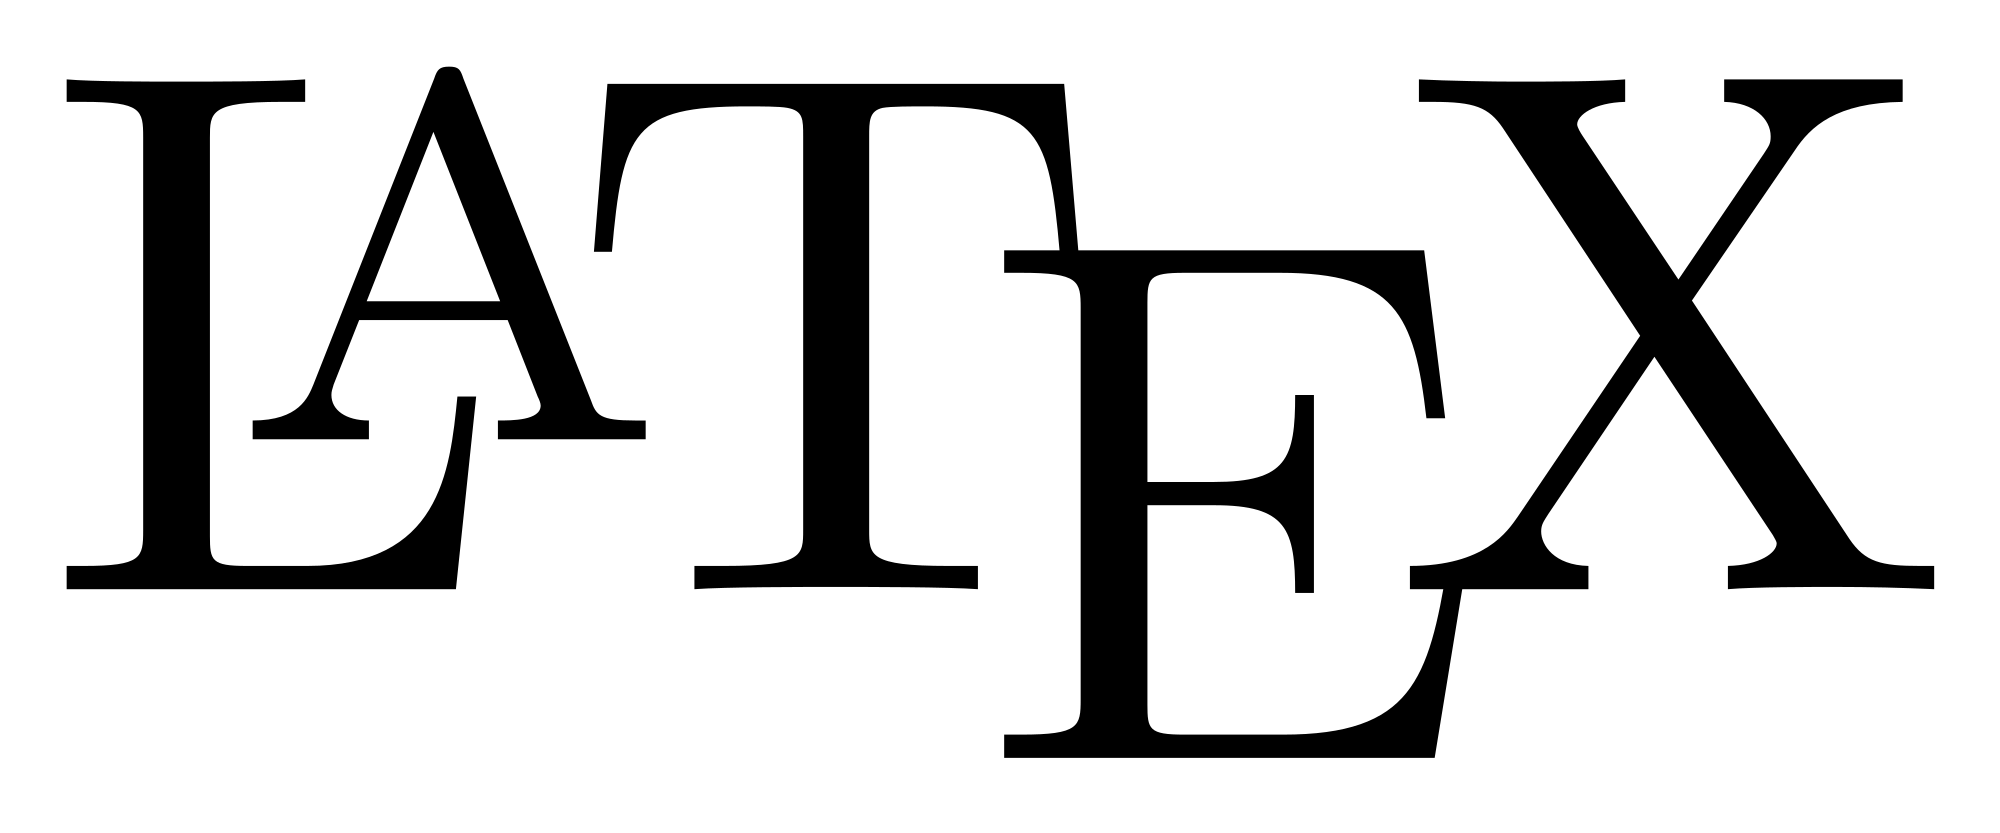
\includegraphics[width=1\textwidth]{img/latex.png}
		\caption{Logo de Latex}
	\end{minipage}
\end{figure}

% ------------------------------------- %
% Introduction au sujet
% ------------------------------------- %

\chapter{Introduction au sujet}

\section{Les réseaux de neurones pronfonds}

Détailer vite fais le fonctionnement du deep learning (Pour qu'un simple lecteur comprenne le fonctionnement de base)

finir par parler de la boite noir.

\section{Jeux de données}

\subsection{MNIST}

\section{Travail à réaliser}

L'objectif du TER est de mieux comprendre le fonctionnement interne d'un réseau de neurones. Concrètement, il s'agit de repérer, selon les données d'entrée, des signatures d'activation de neurones. Pour cela, nous devons répondre aux questions telles que :

\begin{itemize}
	\item Si le jeu d'apprentissage ne contient que des 1 et des 3 quels sont les neurones qui sont activés ?
	\item Existe-t-il des signatures caractéristiques de certaines données ?
	\item A partir de quelle couche le modèle change de comportement pour reconnaître une valeur ?
\end{itemize}

Dans un premier temps, on doit se familiariser avec la base de données MNIST et développer plusieurs outils afin de les manipuler. Ensuite, nous passerons à la construction des modèles d'apprentissage pour pouvoir analyser leurs comportements internes en récupérant les soties de chaque couche cachée. Enfin, nous réaliserons une interface de visualisation afin d'analyser les résultats.

\section{Technologies utilisées}

\subsection{Jupyter notebook}

\subsection{Keras}

% ------------------------------------- %
% Analyse des données
% ------------------------------------- %

\chapter{Analyse des données}

% ------------------------------------- %
% Développement
% ------------------------------------- %

\chapter{Développement de l’architecture}

\section{Modèles d'apprentissage}

\section{Extraction des signatures}

\section{Interface de visualisation}

% ------------------------------------- %
% Analyse des résultats
% ------------------------------------- %

\chapter{Analyse des résultats}

% ------------------------------------- %
% Annexes
% ------------------------------------- %

\appendix
\chapter{Annexe}

\section{...}

\section{...}

\chapter{Bibliographie}


\end{document}
